%%%%%%%%%%%%%%%%%%%%%%%%%%%%%%%%%%%%%%%%%
% Thesis 
% LaTeX Template
% Version 1.3 (21/12/12)
%
% This template has been downloaded from:
% http://www.latextemplates.com
%
% Original authors:
% Steven Gunn 
% http://users.ecs.soton.ac.uk/srg/softwaretools/document/templates/
% and
% Sunil Patel
% http://www.sunilpatel.co.uk/thesis-template/
%
% License:
% CC BY-NC-SA 3.0 (http://creativecommons.org/licenses/by-nc-sa/3.0/)
%
% Note:
% Make sure to edit document variables in the Thesis.cls file
%
%%%%%%%%%%%%%%%%%%%%%%%%%%%%%%%%%%%%%%%%%

%----------------------------------------------------------------------------------------
%	PACKAGES AND OTHER DOCUMENT CONFIGURATIONS
%----------------------------------------------------------------------------------------

\documentclass[11pt, a4paper, oneside]{Thesis} % Paper size, default font size and one-sided paper

\graphicspath{{./Pictures/}} % Specifies the directory where pictures are stored

% Packages 
\usepackage[]{algorithm2e}
\usepackage{algpseudocode}

\usepackage[square, numbers, comma, sort&compress]{natbib} % Use the natbib reference package - read up on this to edit the reference style; if you want text (e.g. Smith et al., 2012) for the in-text references (instead of numbers), remove 'numbers' 
\hypersetup{urlcolor=blue, colorlinks=true} % Colors hyperlinks in blue - change to black if annoying
\title{\ttitle} % Defines the thesis title - don't touch this

\begin{document}

\frontmatter % Use roman page numbering style (i, ii, iii, iv...) for the pre-content pages

\setstretch{1.3} % Line spacing of 1.3

% Define the page headers using the FancyHdr package and set up for one-sided printing
\fancyhead{} % Clears all page headers and footers
\rhead{\thepage} % Sets the right side header to show the page number
\lhead{} % Clears the left side page header

\pagestyle{fancy} % Finally, use the "fancy" page style to implement the FancyHdr headers

\newcommand{\HRule}{\rule{\linewidth}{0.5mm}} % New command to make the lines in the title page

% PDF meta-data
\hypersetup{pdftitle={\ttitle}}
\hypersetup{pdfsubject=\subjectname}
\hypersetup{pdfauthor=\authornames}
\hypersetup{pdfkeywords=\keywordnames}

%Packages


%----------------------------------------------------------------------------------------
%	TITLE PAGE
%----------------------------------------------------------------------------------------

\begin{titlepage}
\begin{center}

\textsc{\LARGE \univname}\\[1.5cm] % University name
\textsc{\Large Masters Thesis}\\[0.5cm] % Thesis type

\HRule \\[0.4cm] % Horizontal line
{\huge \bfseries \ttitle}\\[0.4cm] % Thesis title
\HRule \\[1.5cm] % Horizontal line
 
\begin{minipage}{0.4\textwidth}
\begin{flushleft} \large
\emph{Author:}\\
\href{http://www.johnsmith.com}{\authornames} % Author name - remove the \href bracket to remove the link
\end{flushleft}
\end{minipage}
\begin{minipage}{0.4\textwidth}
\begin{flushright} \large
\emph{Supervisor:} \\
\href{http://www.jamessmith.com}{\supname} % Supervisor name - remove the \href bracket to remove the link  
\end{flushright}
\end{minipage}\\[3cm]
 
\large \textit{A thesis submitted in fulfilment of the requirements\\ for the degree of \degreename}\\[0.3cm] % University requirement text
\textit{in the}\\[0.4cm]
\groupname\\\deptname\\[2cm] % Research group name and department name
 
{\large \today}\\[4cm] % Date
%\includegraphics{Logo} % University/department logo - uncomment to place it
 
\vfill
\end{center}

\end{titlepage}

%----------------------------------------------------------------------------------------
%	DECLARATION PAGE
%	Your institution may give you a different text to place here
%----------------------------------------------------------------------------------------

\Declaration{

\addtocontents{toc}{\vspace{1em}} % Add a gap in the Contents, for aesthetics

I, \authornames, declare that this thesis titled, '\ttitle' and the work presented in it are my own. I confirm that:

\begin{itemize} 
\item[\tiny{$\blacksquare$}] This work was done wholly or mainly while in candidature for a research degree at this University.
\item[\tiny{$\blacksquare$}] Where any part of this thesis has previously been submitted for a degree or any other qualification at this University or any other institution, this has been clearly stated.
\item[\tiny{$\blacksquare$}] Where I have consulted the published work of others, this is always clearly attributed.
\item[\tiny{$\blacksquare$}] Where I have quoted from the work of others, the source is always given. With the exception of such quotations, this thesis is entirely my own work.
\item[\tiny{$\blacksquare$}] I have acknowledged all main sources of help.
\item[\tiny{$\blacksquare$}] Where the thesis is based on work done by myself jointly with others, I have made clear exactly what was done by others and what I have contributed myself.\\
\end{itemize}
 
Signed:\\
\rule[1em]{25em}{0.5pt} % This prints a line for the signature
 
Date:\\
\rule[1em]{25em}{0.5pt} % This prints a line to write the date
}

\clearpage % Start a new page

%----------------------------------------------------------------------------------------
%	QUOTATION PAGE
%----------------------------------------------------------------------------------------

\pagestyle{empty} % No headers or footers for the following pages

\null\vfill % Add some space to move the quote down the page a bit

\textit{``Thanks to my solid academic training, today I can write hundreds of words on virtually any topic without possessing a shred of information, which is how I got a good job in journalism."}

\begin{flushright}
Dave Barry
\end{flushright}

\vfill\vfill\vfill\vfill\vfill\vfill\null % Add some space at the bottom to position the quote just right

\clearpage % Start a new page

%----------------------------------------------------------------------------------------
%	ABSTRACT PAGE
%----------------------------------------------------------------------------------------

\addtotoc{Abstract} % Add the "Abstract" page entry to the Contents

\abstract{\addtocontents{toc}{\vspace{1em}} % Add a gap in the Contents, for aesthetics

The Thesis Abstract is written here (and usually kept to just this page). The page is kept centered vertically so can expand into the blank space above the title too\ldots
}

\clearpage % Start a new page

%----------------------------------------------------------------------------------------
%	ACKNOWLEDGEMENTS
%----------------------------------------------------------------------------------------

\setstretch{1.3} % Reset the line-spacing to 1.3 for body text (if it has changed)

\acknowledgements{\addtocontents{toc}{\vspace{1em}} % Add a gap in the Contents, for aesthetics

The acknowledgements and the people to thank go here, don't forget to include your project advisor\ldots
}
\clearpage % Start a new page

%----------------------------------------------------------------------------------------
%	LIST OF CONTENTS/FIGURES/TABLES PAGES
%----------------------------------------------------------------------------------------

\pagestyle{fancy} % The page style headers have been "empty" all this time, now use the "fancy" headers as defined before to bring them back

\lhead{\emph{Contents}} % Set the left side page header to "Contents"
\tableofcontents % Write out the Table of Contents

\lhead{\emph{List of Figures}} % Set the left side page header to "List of Figures"
\listoffigures % Write out the List of Figures

\lhead{\emph{List of Tables}} % Set the left side page header to "List of Tables"
\listoftables % Write out the List of Tables

%----------------------------------------------------------------------------------------
%	ABBREVIATIONS
%----------------------------------------------------------------------------------------

\clearpage % Start a new page

\setstretch{1.5} % Set the line spacing to 1.5, this makes the following tables easier to read

\lhead{\emph{Abbreviations}} % Set the left side page header to "Abbreviations"
\listofsymbols{ll} % Include a list of Abbreviations (a table of two columns)
{
\textbf{LAH} & \textbf{L}ist \textbf{A}bbreviations \textbf{H}ere \\
%\textbf{Acronym} & \textbf{W}hat (it) \textbf{S}tands \textbf{F}or \\
}

%----------------------------------------------------------------------------------------
%	PHYSICAL CONSTANTS/OTHER DEFINITIONS
%----------------------------------------------------------------------------------------

\clearpage % Start a new page

\lhead{\emph{Physical Constants}} % Set the left side page header to "Physical Constants"

\listofconstants{lrcl} % Include a list of Physical Constants (a four column table)
{
Speed of Light & $c$ & $=$ & $2.997\ 924\ 58\times10^{8}\ \mbox{ms}^{-\mbox{s}}$ (exact)\\
% Constant Name & Symbol & = & Constant Value (with units) \\
}

%----------------------------------------------------------------------------------------
%	SYMBOLS
%----------------------------------------------------------------------------------------

\clearpage % Start a new page

\lhead{\emph{Symbols}} % Set the left side page header to "Symbols"

\listofnomenclature{lll} % Include a list of Symbols (a three column table)
{
$a$ & distance & m \\
$P$ & power & W (Js$^{-1}$) \\
% Symbol & Name & Unit \\

& & \\ % Gap to separate the Roman symbols from the Greek

$\omega$ & angular frequency & rads$^{-1}$ \\
% Symbol & Name & Unit \\
}

%----------------------------------------------------------------------------------------
%	DEDICATION
%----------------------------------------------------------------------------------------

\setstretch{1.3} % Return the line spacing back to 1.3

\pagestyle{empty} % Page style needs to be empty for this page

\dedicatory{For/Dedicated to/To my\ldots} % Dedication text

\addtocontents{toc}{\vspace{2em}} % Add a gap in the Contents, for aesthetics

%----------------------------------------------------------------------------------------
%	THESIS CONTENT - CHAPTERS
%----------------------------------------------------------------------------------------

\mainmatter % Begin numeric (1,2,3...) page numbering

\pagestyle{fancy} % Return the page headers back to the "fancy" style

% Include the chapters of the thesis as separate files from the Chapters folder
% Uncomment the lines as you write the chapters

\setstretch{2} % Return the line spacing back to 1.3

\chapter{Background} % Main chapter title

\label{Background} % For referencing the chapter elsewhere, use \ref{Chapter1} 

\lhead{Chapter 2. \emph{Background}} % This is for the header on each page - perhaps a shortened title

\section{Nearest Neighbors Search}

\subsection{Overview}
\label{sec:overview}

One common way to represent a collection of objects is as a set of points in a vector space with a fixed number of dimensions.  Each object is represented as a vector, or point, in the vector space, and each dimension in the vector space represents a different feature of the object.  The distance between two points in a vector space is analagous to the relatedness of two objects.  Nearest neighbors search aims to find the closest points to a query point in a vector space.  This type of search has a variety of applications in pattern recognition \citep{cover1967nearest}, information retrieval \citep{manning2008introduction} and computer vision \citep{boiman2008defense}.

There are a variety of different types of vector spaces such as boolean valued, integer valued and mixed; however, we will focus on real-valued vector spaces.  In these spaces, the value of every dimension in a vector can be expressed as a real number.  Closeness can be defined by a variety of different distance metrics.  Some common distance metrics between two N-dimensional points, x and y, are shown in Table \ref{table:distancemet}.  In low dimensional spaces, the Euclidean distance is typically used \citep{danielsson1980euclidean}, and will be the focus of future sections.

\begin{table}
\centering
\begin{tabular}{ | l | c |}
	\hline
	Distance Type & Distance Function \\
	\hline
	Euclidean & $\sqrt{\sum\limits_{i=1}^N (x_i - y_i)^2}$ \\
	\hline
	Manhattan & $\sum\limits_{i=1}^N |x_i - y_i|$ \\
	\hline
	Chebyshev & $\max{|x_i - y_i|}$ \\
	\hline
\end{tabular}
\caption{Distance Metrics}
\label{table:distancemet}
\end{table}

\subsection{Basic Search Algorithm}
\label{sec:linear}

The most basic algorithm for a nearest neighbor search performs a linear scan across every element in a set.  Such a method computes the distance between a query point and every single point in a dataset, and returns the point with the minimum distance.  For a dataset with N points of dimensionality D, the complexity of this operation is O(ND).  For large datasets this linear time approach is not feasable, especially if many queries need to be performed.

\subsection{K-nearest Neighbors}
\label{subsec:knn}

The basic linear search algorithm can easily be extended to support a query which returns the k-nearest neighbors rather than simply the closest.  This change requires the use of a priority queue.  A priority queue guarantees amortized O(log(N)) insert and delete-max operations and constant time check-max \citep{van1976design}.  Certain implementations of a priority queue allow even faster guarantees.  For example, for binary heaps allow for average case constant time and worst case logarithmic insertion \citep{carlsson1988implicit}.  The priority metric for points will be their distance to the query point.  The first K points searched are automatically added to the priority queue.  For future points searched, if a point is closer than the furthest of the top K, the delete-max operation can be performed, and the new closer point can be added to the priority queue ensuring that K elements always remain.  If the most recently checked point is not one of the top K, then only the constant time check-max operation needs to be performed.  If the point is closer than one of the top K, the delete-max and insert operations must be performed as well.  Because both of those operations are logarithmic, the cost of updating the priority queue will at most be O(log(K)).  In practice, however, the priority queue is updated very rarely.  Assuming the points are searched in random order, the probability that a point being processed will be one of the current top K encountered is relatively low.

The k-nearest neighbors (k-NN) result is extremely useful for classification and regression on labeled datasets.  For a classification task one common way to make a hard decision on a class is to use the class that appears most frequently in the top K.  Thus, for datasets where test data is very similar to training data, this simple inference method can perform extremely well.  k-NN can also be used for regression.  Since the output is continuous in this case, the average of the results in the top K can be used.

The k-nearest neighbors has a few limitations, however \citep{beyer1999nearest}.  For one, it is an instance based learning technique.  This means that it will only perform well when instances are similar to those from training and thus does not generalize well \citep{aha1991instance}.  Another issue is the computational cost of this method.  While no training is required, each k-NN query requires linear time with respect to the size of the dataset.  Approximate nearest neighbors described in \ref{sec:ann} attempts to address this.  Another issue is that common distance metrics, such as Euclidean distance, weight each dimension equally.  Thus, in order to achieve reasonable results one must normalize all dimensions.

\section{Fixed Radius Search}

Another common search type is a fixed radius search \citep{dickerson1990fixed}.  This type of search attempts to find all points within a distance R of a query point.  The linear search algorithm can easily be adapted to this type of query.  After computing the distance between the query point and each point in the training set, if this distance is found to be less then R that point can be added to the result set.

\section{Approximate Nearest Neighbors}
\label{sec:ann}

Computation of the exact nearest neighbors via a linear search algorithm is extremely costly.  One way to improve this performance is to create an index.  The goal of an index is to increase the speed of a nearest neighbors query at the cost of additional preprocessing time and memory.  In low dimensional spaces, one common index is the k-d tree described in more detail in Section \ref{sec:kdtree}.  While the k-d tree supports average case O(log(N)) queries in low dimensional spaces, no index has beeen found which is guaranteed to return the exact set of neighbors in linear time \citep{muja_flann_2009}.

However, for many applications it is not important that the result set be perfectly accurate.  It may be advantageous to return a set which isn't guaranteed to be exact in significantly less time. For these reasons, approximate nearest neighbors are often computed instead of exact nearest neighbors.  The most common index types for approximate nearest neighbor algorithms are constructed out of trees, hash tables, or graphs \citep{flann_pami_2014}.

\subsection{Tree Based Indexes}
\label{sec:treeind}

The main concept behind a tree based index is space paritioning.  As such, these types of indexes tend to be extremely effective in low dimensionality settings, but do not scale as well to those of higher dimensionality.  Generally, at the root of these indexes, the entire search space is present \citep{yianilos1993data}.  As the tree splits, space is partitioned and only points which satisfy a split criteria will be present in each subtree.  Thus, when searching to the leaf of these trees, one can find the space partition a query point lies in, and by recursively backtracking, a process similar to the one described for k-d trees in Section \ref{sec:kdtree} can gradually expand the search radius.  K-d trees, described in detail in Section \ref{sec:kdtree}, are one of the most widely used tree based indexes.  The main advantages of k-d trees are that they are relatively fast to construct, can be easily modified, and have worst case linear space consumption \citep{yianilos1993data}.

K-means trees are another type of tree often used in practice \citep{flann_pami_2014}.  These trees are constructed with a branching factor K.  At each node, the k-means clustering algorithm is perfomed, separating remaining points into K clusters \citep{hartigan1979algorithm}.  This branching continues until less than K points remain in a node, at which point the node becomes a leaf.  To search a tree, one can move to a leaf by moving down the tree selecting the cluster with the closest mean to the query point.  As the search proceeds, each cluster's center is added to a priority queue, with its priority set as the distance from the query point.  When a leaf is reached the algorithm continues the search at the closest center in the priority queue.

K-means trees are more expensive to construct than k-d trees, as the K-means algorithm is not guaranteed to converge quickly.  Additionally, since all points are stored in the leafs and only cluster centers are stored at each node, the tree will be larger.  K-means trees, however, tend to be more effective than k-d trees when high precision is required in the result set.

Quad trees are another algorithm commonly used for nearest neighbor searches \citep{finkel1974quad}.  In a two dimensional space, each point in a quad tree splits space into 4 different quadrants, similar to how the origin separates a standard x and y axis into four regions.  The tree will be expanded this way and as such has a higher branching factor than k-d trees leading to lower depth.  Quad trees can also be expanded into octrees for 3-D space and generalized into similar higher orders for even higher dimensionality \citep{samet1988overview}.  Unfortunately, in higher dimensional spaces of dimensionality D, each point splits space into $2^D$ regions.  This often leads to many unused pointers since points will not likely lie in all of these regions.  As such, the memory cost of quad tree variants can become extremely large.

\subsection{Hash Indexes}
\label{sec:hashind}

Many variations of hash indexes exist; however, the most widely used is locality-sensitive hashing (LSH).  The goal of LSH is to use a variety of different hash functions to map similar points into the same buckets.  Rather than using cryptographic hash functions which map entities into a bucket independent of their state, the hash functions used in LSH aim to match similar points into the same bucket with a high probability, and dissimilar points into the same bucket with a low probability.  Formally, each hash function maps a D-dimensional vector v into one of R buckets \citep{datar2004locality}.  Many different types of hash functions can be used, such as projection, lattice, and quantization-based hash functions.  Different types of hash functions have been studied and evaluated extensively \citep{pauleve2010locality}.

Thus, to initialize an LSH index, one must pass every point through H hash functions, and store a key to each point within every bucket it falls into.  A larger H leads to more information in the results however requires more processing time and memory consumption.  Additionally, since all the information becomes compressed into these hash functions, these types of indexes generalize well to higher dimensional spaces.

To query an LSH index one must pass a query point through all H hash functions, and search each bucket for collisions.  The entries that most commonly collide have a smaller hamming distance in the new hash space, and will thus be treated as the most similar points.

While LSH scales extremely well to high dimensional spaces, one disadvantage is that its memory consumption tends to be much larger than that of tree based indexes in low dimensional spaces \citep{datar2004locality}.  Another key disadvantage is that quality of the search queries cannot be changed, as this is dependent on H and R.  In other words, LSH indexes have their maximum accuracy constrained during their construction, wheras tree based indexes can have variable levels of accuracy on each query dependent on the number of nodes searched.

\subsection{Graph Indexes}
\label{sec:graphind}

Graph based indexes tend to be the most expensive type to construct; however, they can support extremely fast queries.  One common type is a k-nearest neighbor graph.  In this type of graph, each node has exactly K edges, in which each node is connected to its k-nearest neighbors.  A variety of different algorithms are available for constructing these types of graphs efficiently \citep{connor2010fast}.

To perform a nearest neighbor query, a very common technique is a greedy traversal of the graph \citep{hajebi2011fast}.  Given a query point, a randomly chosen node in the graph is chosen as the startpoint.  Each neighbor is checked, and the next node traversed to is the one which is closest to the query point.  The algorithm is terminated after a fixed number of moves, where a higher number of moves will have improved results.  The K best nodes encountered are returned as the k-nearest neighbors.  Often times random resets are incooperated to ensure that different parts of the graph are searched.  Another common heuristic is to only search a randomly selected subset of the connected nodes at each node.

From experimental results, these indexes tend to perform better than LSH and k-d trees \citep{hajebi2011fast}.  However, one downside is that the offline construction of the graph is very expensive.  Additionally, there is a large amount of randomness in the search algorithm, so there tends to be a large variance in the quality of the results obtained from queries with the same point.

\section{k-d Trees}
\label{sec:kdtree}

\subsection{Overview}
The k-d tree was originally developed as ``a data structure for storage of information to be retrieved by associative searches'' \citep{bentley1975multidimensional}. k-d trees are efficient both in the speed of associative searches and in their storage requirements.  A k-d tree is a binary tree which stores points in a d-dimensional space.  Each node contains a single d-dimensional point, a split dimension, and up to two children nodes.  Each node represents a hyperplane which lies perpendicular to the split dimension and passes through the stored point.  The left subtree of a node contains all points which lie on one side of the hyperplane, while the right subtree represents all points which lie on the other side of the hyperplane.  Thus, each node partitions all nodes below it into two half-spaces.  Because only a single split dimension is used at each internal node, each splitting hyperplane is axis-aligned.  This splitting procedure continues on each subtree until each node contains only one element.  The procedure for axis selection on each split is described in section \ref{subsec:const}.

\subsection{Construction}
\label{subsec:const}

\begin{figure}
\setstretch{2}
\begin{algorithmic}
\Function{kdtree}{pointList}
	\If {pointList is empty}
		\State \Return null
	\EndIf
	\State splitDim = selectAxis()
	\State
	\State medianPoint = selectMedian(pointList, splitDim)
	\State remove medianPoint from pointList
	\State initialize empty leftList, rightList
	\ForAll{points p in pointList}
		\If {p(splitDim) $<$ medianPoint(splitDim)}
			\State leftList.Add(p)
		\ElsIf{p(splitDim) $>$ medianPoint(splitDim)}
			\State rightList.Add(p)
		\Else
			\State randomly add p to leftList or rightList with equal probability
		\EndIf
	\EndFor
	\State
	\State treenode node = new treenode()
	\State node.splitDim = splitDim
	\State node.splitPoint = medianPoint
	\State node.leftChild = kdtree(leftList)
	\State node.rightChild = kdtree(rightList)
	\State \Return node
\EndFunction
\end{algorithmic}
\caption{Pseudo code for Constructing a k-d tree}
\label{alg:createkd}
\end{figure}

The construction of a k-d tree is performed recursively with input parameters of a list of points.  Pseudo code is shown in Figure \ref{alg:createkd}.  Axis selection can be performed in multiple ways.  The classical approach is to deterministically iterate between all N dimensions.  Another approach, known as spatial median splitting, selects the the longest dimension present in the current pointList to split on \citep{zhou2008real}.  The downside of this method is that a linear traversal is required to select the split dimension.  Another popular approach is to randomly select the split dimension with an equal probability of selecting each dimension.  This approach is often applied when using multiple k-d trees; because of the additional randomness, trees are likely to be different \citep{flann_pami_2014}.  While a linear time algorithm for determining the median of an unordered set is possible \citep{megiddo1984linear}, a heuristic approach is typically used to approximate the median.  A common heuristic is to take the median of five randomly chosen elements; However many other methods can be used such as the triplet adjust method \citep{battiato2000efficient}.

At the termination of the algorithm, the root of the k-d tree is returned, and each node contains exactly one point.  The runtime of this algorithm has an average case O(Nlog(N)) running time where N is the number of points in pointList.  While the median can be approximated in constant time, partitioning pointList along that median is an O(N) operation.  Since the k-d tree is a binary tree in which each node holds one point, assuming it is relatively balanced, its height is O(log(N)).  Another key point is that points which match medianPoint along splitDim should be randomly assigned to a subtree.  This will ensure that if many points have the same value along a given dimension all of these points will be distributed close to evenly between the two subtrees allowing the tree to remain balanced.

\subsection{Nearest Neighbor Query}
\label{sec:kdquery}

A simple algorithm exists to apply the k-d tree to a nearest neighbor query.  This algorithm is guaranteed to find the single closest point to the search query.  Pseudocode for this algorithm is shown in Figure \ref{alg:querykd}.  The inputs to this algorithm are the root of the tree, the query point, and dummy current best point located at infinity in each dimension.

\begin{figure}
\setstretch{2}
\begin{algorithmic}
\Function{searchkdtree}{node, searchPoint, currBest}
	\If{node is a leaf}
		\If{dist(node.splitPoint, searchPoint) $<$ dist(currBest, searchPoint)}
			\State currBest = node.SplitPoint
		\EndIf
		\State \Return
	\EndIf
	\State
	\State dim = node.splitDim
	\State Boolean searchDir = searchPoint[dim] $<$ node.splitPoint[dim]
	\State searchFirst = searchDir ? node.left : node.right
	\State searchSecond = searchDir ? node.right : node.left
	\State searchkdtree(searchFirst, searchPoint, currBest)
	\State
	\If{dist(node.splitPoint, searchPoint) $<$ dist(currBest, searchPoint)}
		\State currBest = node.SplitPoint
	\EndIf
	\If{HyperPlaneCheck(searchPoint, currBest, searchSecond)}
		\State searchkdtree(searchSecond, searchPoint, currBest)
	\EndIf

\EndFunction
\end{algorithmic}
\caption{Pseudo code to apply a nearest neighbor search using a k-d tree}
\label{alg:querykd}
\end{figure}

The first part of the algorithm recursively steps down the tree until a leaf is reached.  At each node, a comparison on the split dimension is performed to determine which side of the splitting hyperplane the search point lies so that the search can continue in the proper half space.  When a leaf is reached, the point stored in the leafnode is set as the current closest point.  The algorithm then recursively walks back up the tree, and at each node computes the difference between the current node's point and the searchpoint.  If this distance is smaller than that of the current best, the current node point becomes the current best.

The algorithm then determines whether a closer point than the current best could potentially exist in the second unsearched subtree.  Because all hyperplanes are axis aligned, this computation is very simple.  The closest possible point in the halfspace represented by the second subtree could potentially lie within a distance of $\epsilon$ from the hyperplane, where $\epsilon$ is very small.  The lower bound of the distance of the closest point, occuring when $\epsilon$ approaches zero, is the absolute value of the difference between the search point and split point along the current split dimension.  If this distance is larger than the current best point's distance, then the algorithm does not need to check the second subtree, as there is no possible closer point in that halfspace.  If this distance is smaller however, then the algorithm will search down the second subtree following the exact same procedure as before, treating the second child as the root.  Because of this comparison however, the worst case running time of this algorithm is O(N), as if all comparisons fail, then the entirity of the tree will be searched.  As the dimensionality of the tree becomes larger, this check is more likely to fail, and k-d trees diminish in effectiveness.

This algorithm can be extended to support KNN with the same priority queue procedure described in Section \ref{subsec:knn}.  The check as to whether a closer point could potentially exist in the second subtree will then be performed against the furthest point in the top K.  This algorithm can also be extended to perform a radius bounded search.  Rather than checking the distance to the hyperplane compared to the furthest point in the top K one can check against a fixed radius R.  Thus, this algorithm can also efficiently find all points within R of the query point.

\subsection{Approximate Nearest Neighbors Query}

The k-d tree nearest neighbor search algorithm can be extended into an approximate nearest neighbors search.  To do so, a limit on the number of points to search must be applied.  The algorithm will follow the exact same steps as shown in Figure \ref{alg:querykd}; however, when the search limit is reached the algorithm terminates.  This means that not every possible node that might contain a closer point would necessarily be searched.  However, the nodes that do get searched are more likely to contain the closer points.  In other words, the algorithm will examine the regions of space which are closest to the search query first before expanding outward.

\subsection{Modification}
\label{sec:kdmod}

One key advantage of k-d trees is that they are very easy to modify.  Inserting a node requires a traversal to a leaf node following the same procedure as described in the first part of Figure \ref{alg:querykd}.  This search takes approximate O(log(N)) time if the tree is balanced.  Once a leaf node is reached, a single comparison along the split dimension needs to be performed in order determine whether the new node should be added as the left or right child.  If random points are inserted on a balanced tree, the tree will remain relatively balanced as there will be an equal probability of placing points below each leaf.  Heuristics can be used to help ensure that a tree remains balanced in a dyanmic environment \citep{hunt2006fast}.

Deletion on k-d trees can also be performed with relative ease.  Again a downward traversal is performed until the target node is encountered. If the target node is a leaf, it can be removed trivially by removing the connection from its parent.  If the target node is not a leaf, lazy deletion can be performed.  The node will not be removed and will still serve to partition space; however it will not store any actual split point against which comparisons can be made.  If many nodes are lazy deleted, performance will slowly degrade, and reconstruction of the tree may be advisable.

\section{Randomized k-d Tree Forests}
\label{sec:randomforest}

With one k-d tree, one runs the risk of potentially very bad queries occuring when one of the earlier splitting hyperplanes lies close to the point of interest.  By having a forest of multiple k-d trees made from randomized split dimensions and splitpoints, the effects of this can be minimized.  \citep{silpa2008optimised} has shown that k-d tree forests can lead to inproved performance.  It is important to note that when searching multiple trees, the same heap must be used, and as such this object needs to properly be mutex locked if the search is to occur in parallel.  As better results are found in each tree, more hyperplane checks will pass and less time will be wasted searching parts of the tree where better results do not lie.  When searching trees sequentially, rather than in parallel, the performance was significantly weaker \citep{silpa2008optimised}.

Another approach to improve performance is the rotation of dimensions along different trees \citep{silpa2008optimised}.  This allows the splitting hyperplanes to no longer be constrained to axis alignment, and can introduce a greater amount of variety in the forest.  Based on experimental results, the optimal amount of trees was generally less than 20, though the number varied greatly between different datasets \citep{muja_flann_2009}.
\chapter{Related Work} % Main chapter title

\label{Related Work} % For referencing the chapter elsewhere, use \ref{Chapter1} 

\lhead{Chapter 2. \emph{Related Work}} % This is for the header on each page - perhaps a shortened title

\section{Approximate Nearest Neighbor Frameworks}

Many ANN frameworks exist for fast computation.  Since no exact nearest neighbors algorithms are faster than linear time in high dimensional spaces, a variety of different ANN algorithms must be applied.  The Fast Library for Approximate Nearest Neighbors (FLANN) makes use of many of these algorithms including k-d trees, k-means trees, and locality sensitive hashing \citep{muja_flann_2009}.  However, each of these types of indexes have different properties, and some may be suited to some datasets more than others.  Thus, one difficult task this framework can perform is automatic selection of the index type and parameters.  This is done by estimating the overall cost of an index in terms of memory consumption, index generation time, and query speed to achieve a given accuracy.  The user of the system can also put weights on each of these costs to raise the relative importance of one ore more of these factors.  By benchmarking on a small subset of a dataset, the framework can effectively select the most efficient index type and apply the simplex optimization algorithm \citep{nelder1965simplex} to optimize its parameters.

Also of importance with FLANN and other frameworks is that they are optimized for real world performance.  This means that that benchmarks are taken in terms of real time, and memory consumption is minimized.  For example, when possible bit array keys are used rather than pointers in order to save as much memory as possible.
\chapter{System Description} % Main chapter title

\label{sysdes} % For referencing the chapter elsewhere, use \ref{Chapter1} 

\lhead{Chapter 3. \emph{System Description}} % This is for the header on each page - perhaps a 

\section{Overview}
\label{sect:sysdesover}

As mentioned in subsection \ref{subsec:knn}, before applying a nearest neighbors algorithm, one must normalize dimensions proportional to their relevance.  Conventionally, if the relevance of a dimension or a set of dimensions were to be changed, one must perform a linear transformation on the every single point in the search space.  When using an index type described in section \ref{sec:ann}, this linear transformation requires a total reconstruction of the index for optimal nearest neighbors search performace, as the distance between all pairs of points in the index is now different.

The goal of this system is to support queries of dynamic dimension relevance in low dimensional spaces.  Dynamic dimension relevance means that requester of a given query must provide both a search point, and the relevance of each dimension in the query.  The system will then compute the ANNs using a modified Euclidean distance metric in which the distance in each dimension is weighted proportionately to the relevance.  This metric is described formally in section \ref{subsec:dimrel}.

\subsection{Normalization}
\label{subsec:normalization}

Each dimension in the vector space representation of a dataset must be normalized to ensure that each dimension is initially weighted equally.  The normalization scheme used performs a linear transform to set the min of a dimension to zero and the max to one.  After finding the min and max of each dimension, one must normalize every dimension of every point following equation \ref{eq:normd}.

\begin{equation}
\label{eq:normd}
d_{normalized} = \dfrac{d-d_{min}}{ d_{max} - d_{min} }
\end{equation}

This normalization technique is ideal for datasets which follow a relatively uniform distribution.  However, the presence of outliers could greatly skew this normalization scheme.  An alternative normalization strategy for these cases is to normalize the mean of each dimension to zero, and the variance to one.  This can be achieved by following the linear transformation outlined in equation \ref{eq:normd2}.  This procedure is equivalent to finding the standard score or z-score of each dimension \citep{cheadle2003analysis}.

\begin{equation}
\label{eq:normd2}
d_{normalized} = \dfrac{d-d_{mean}}{ d_{stdev} }
\end{equation}

\subsection{Dimension Relevance}
\label{subsec:dimrel}

After normalization described in section \ref{subsec:normalization}, each dimension in the dataset is said to have equal relevance, and would have an equivalent contributribution to a standard Euclidean distance.  As described in section \ref{sect:sysdesover} each query requires both a search point, and a dimension relevance vector (DRV).

The DRV must contain the same number of dimensions as all points in a dataset.  Each element in the DRV contains a weight on each dimension.  The DRV is then normalized to have a sum of one.  Using the DRV v and two D dimensional points x and y, the modified Euclidean distance metric is shown in equation \ref{eq:eucmod}.

\begin{equation}
\label{eq:eucmod}
distance = \sqrt{\sum\limits_{i=1}^D ((x_i - y_i) \times v_i \times D)^2)} \\
\end{equation}

For the case in which all dimensions are weighted equally, each element is $v_i=1/D$.  Thus, in this special case, the standard Euclidean distance is computed.  This distance metric is also equivalent to transforming each dimension via multiplying by $v_i \times D$, and computing the standard Euclidean distance.  By using this modified metric instead, this transformation does not need to be explicitly performed but is inherent in the distance calculation.

\subsection{Motivation for k-d Trees}

We aim to tackle the the challenge of creating an ANN index which performs well when DRVs are specified at query time, and allows for queries of different quality requirements.  We opted to base our index on k-d trees for a variety of different reasons.  Graph indices, as described in \ref{sec:graphind} have a high offline construction cost, and compute the KNN of each node at construction time.  This makes them poorly suited to adapt to a changing distance metrics.  Hash based indexes, described in \ref{sec:hashind} also have some downsides.  Generally, the hash functions used act as quantizers and aren't tied directly to dimensions in a vector space.  Additionally, the accuracy of hash based indexes is tied to the number of hash functions, and the amount of buckets of each.  As such this quality cannot be changed at query time.

Tree based indexes, described in \ref{sec:treeind} tend to be the most memory efficient in low dimensional spaces.  Additionally, the partitioning of tree indexes is inherentaly tied to the vector space representation.  A specific advantage of k-d trees, described in \ref{sec:kdtree} is that they are guaranteed to be linear in size, and splits can only occur orthogonal to a dimension.

\subsection{Split Dimension Determination Heuristics}
\label{section:splitdim}

A common heuristic for determining the split dimension on k-d tree indexes is spatial median splitting (SMS) \citep{zhou2008real} \citep{wald2006building}.  SMS always selects the longest dimensions as the one to be split on.  The motivation for this technique is that each hyperrectangle should be as close to a cuboid as possible.  In doing so, the check of whether or not a ball of radius R around a point intersects with an enclosing hyperplane is more likely to result in no intersection.  When no intersection occurs the k-d tree search algorithm described in section \ref{sec:kdquery}, can eliminate a subtree without searching it.  It is important to note that k-d trees can still function, even if the partitions are not square.  However, because of the inability to prune subtrees as effectively, ANN searches will not be as efficient, and the quality of the result set under the constraint of a fixed number of searches will suffer.  It is also important to note that on a vector space in which each dimension has been normalized, selecting a random dimension to split on with equal probability accomplishes a similar effect to SMS.  On average, regions will tend to be close to cuboids. The advantage of this method is less offline computation in index construction and more variety in trees.  This additional variety is advantageous when searching multiple trees \citep{flann_pami_2014}.

When applying dimension weights via a DRV to a k-d tree search, the distance metric acts on a transformed space.  As such, if the split dimension is selected with SMS or randomly with equal probability on each dimension, the regions would no longer be cuboids on average.  Two different possible heuristics are applied to combat this.  The first is split probability matching (SPM).  The goal of this heuristic is to adjust the probability of splitting on each dimension to account for the fact that in the transformed space the dimensions are no longer normalized to the same weight.  Therefore, by selecting split dimensions with probabilities equal to the weight of each dimension, the regions will tend to approach a cuboid shape in the transformed space.  The second heurstic is weighted spatial median splitting (WSMS).  WSMS is performed the same way as SMS, however the distance between the max and min of dimension is multiplied by the dimension weight from the DRV.  Thus, this technique is equivalent to SMS on the transformed vector space.

\subsection{Initial Tests}

Figures \ref{fig:drvmatching} and \ref{fig:drv_varying_points}, demonstrate the effectiveness of both of these heuristics in improving the quality of ANN perfomance when applying a DRV.  The dataset used for these tests was 100,000 8 dimensional points, in which the value for each dimension is pulled from U(0,1).  100 different randomly generated DRVs were generated via applying U(0,1) in each dimension and normalizing to a sum of one.  10 query points were generated for each DRV following the same procedure from the generation of the dataset.  Thus, this test consists of 1000 queries on each index type.  For this test K was set to 50, while the max number of searches was set to 500.

Initially two k-d trees were generated.  One used SMS as its split dimension selection method, while the other selected randomly.  Additionally, a forest of three trees was generated in which each tree used SMS to selected split dimensions, while the other selected randomly.  For each of the generated DRVs, four new indexes were created.  A tree using WSMS, a tree using SPM, a forest of 3 trees using WSMS on each and a forest of three trees using SPM on each.

A standard linear search was applied using the modified distance metric to determine the correct top K for each DRV and query point.  An ANN query was then performed using the eight different indexes (four of which are the same across all query points, while four were initialized using the seed DRV for each of the 100 seed DRVs).  The evaluation metric used is mean percent distance gain (MPDG).  The average distance of each set of K elements was calculated.  Then, using equation \ref{eq:evalmetric} the average distance in each ANN set was compared to that of the linear search.  A gain in this average distance represents a lower quality result.  Figure \ref{fig:drvmatching} displays the results of these initial tests.  A single k-d tree using WSMS had the highest performance.  Spatial median splitting and its variant tended to perform better than the randomized methods, and single trees performed better than forests.

\begin{equation}
\label{eq:evalmetric}
MPDG = average\_distance_{index} / average\_distance_{linear} - 1 \\
\end{equation}

\begin{figure}[h]
\begin{center}
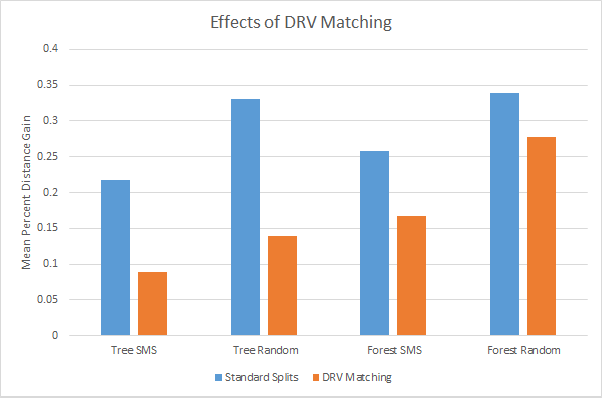
\includegraphics[width=\textwidth]{Figures/sysdesc_drvmatching}
\end{center}
\caption{Initial tests of DRV matching heuristics}
\label{fig:drvmatching}
\end{figure}

Figure \ref{fig:drvmatching}, shows a similar test with a varying number of points searched.  This figure however only includes the first results for a standard k-d tree using SMS and the variant using WSMS.  From this plot it can be seen that WSMS has significantly better performance with a low number of points searched, and eventually both SMS and WSMS converge to very accurate results given enough searches.  Another perspective which can be made from this plot is that under the constraint of a minimum quality, for any quality chosen, WSMS will return the result significantly faster.  For example, if a MPDG of .15 is required, WSMS would reach that level of quality approximately three times faster.  Thus, from these plots it is clear that both of these heuristics have the potential for better results.  Further evaluations are performed in chapter \ref{results} to determine scenarios in which both of these heuristics are most effective.

\begin{figure}[h]
\begin{center}
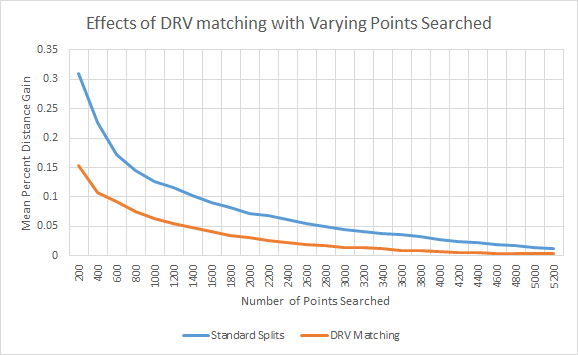
\includegraphics[width=\textwidth]{Figures/sysdesc_drv_varying_points}
\end{center}
\caption{Effects of DRV matching in a single k-d tree using SMS/WSMS with varying number of points searched}
\label{fig:drv_varying_points}
\end{figure}

\subsection{Tree Quality Metric}

While SPM and WSMS can result in greatly improved ANN performance, these methods are not directly feasible in practice on a system which supports specifying a DRV at query time rather than during tree construction.  As shown in section \ref{subsec:const} the cost of generating a k-d tree is Nlog(N), while the cost of a standard linear query is N.  Thus, generating new trees to directly match the DRV of each query is not practical, as the tree construction cost is higher than a that of a linear search.

To work around this, we opted to construct a large set of k-d trees from a variety of different seed DRVs, whose selection process is detailed in section \ref{sec:myalgconst}.  On each query, our index can then select the tree or subset of trees whose seed DRVs best match the queries's DRV.  In doing so, the set of trees searched will have been generated based on DRVs similar to that of the query, leading to improved performance for ANN queries.

The quality metric of a tree used is the modified Euclidean distance metric from equation \ref{eq:eucmod}.  Rather than comparing two points however, the two entities compared are the query DRV and the seed DRV of a tree, both of which have been normalized to have a sum of one.  The set of trees with the highest quality (smallest distance) can then be searched in parallel.  Additionally, based on the result of this tree quality metric, the parallel search between multiple trees can be skewed towards the trees of highest quality, searching these trees more deeply.

There is of course a tradeoff between the size of the set of k-d trees, and system performance.  More trees will result in high quality matches for more DRVs, and thus improved accuracy.  However, each additional tree is linear in memory consumption, so the number of these trees must be kept within reason.  Additionally, each test of the tree quality metric is computationally equivalent to a comparison between two points.  As such, the cost associated with computing the quality metric of each tree which must be accounted for in performance benchmarks.

\section{Detailed Implementation Overview}
\label{sec:myimpl}

\subsection{Index Construction}
\label{sec:myalgconst}

The initial dataset input into the system is an unordered set of N points containing D dimensions.  The first step is to normalize all points in this set along each dimension using the scheme specified in equation \ref{eq:normd} or \ref{eq:normd2}, per selection of the user.  The user must also select their split dimension heuristic to be SPM or WSMS as described in section \ref{section:splitdim}.  Both heuristics are evaluated in chapter \ref{results}.

The user also needs specify two index size parameters: the deterministic dimension depth (DDD), and the number of random trees.  Both of these parameters impact the number of trees which will be generated.  The use of the DDD allows the system to perform well on DRVs which put very heavy weight on a low number of dimensions, which is likely to be common in practice.  To do so, a tree is generated with every possible subset of dimensions containing less than or equal to the DDD.  In each of these subsets, the seed DRV has equal weight in each of these dimensions, and as such are equivalent to $1/D$.  The number of trees needed to satisfy a DDD of R on a dataset with dimensionality D is shown in equation \ref{eq:ddd}.  This number scales factorially with both D and R, so a very small R must be used if D is large to ensure that the number of trees is reasonable.  A large R however has the advantage of high quality tree matches on queries with R or less dimensions.

\begin{equation}
\label{eq:ddd}
ntrees = \sum\limits_{i=1}^R {D \choose i}
\end{equation}

The number of random trees directly controls the number of trees generated with seed DRVS pulled from a uniform distribution.  Each initial weight on each dimension is a number selected randomly from U(0,1) on each dimension, and the results are normalized to have a sum of one.  A larger number of random trees will result in overall better matches on randomly selected DRVs at the cost of memory consumption.  Other types of dimension split priors other than uniform could be used instead if additional information was known about the distribution of DRVs used.  This possiblity is further considered in chapter \ref{conclusion}

The total number of trees generated is the number of deterministic trees as specified by equation \ref{eq:ddd} combined with the number of random trees.  A final tree is also added which is seeded from a uniform DRV to perform standard ANN queries.  Each tree is generated following the algorithm in section \ref{subsec:const} with the modification that the split dimension is selected via SPM or WSMS rather than from a uniform distribution.  Implementation details about weighted random number selection are described in \ref{sec:rng}.  In our test environment, if the number of trees exceeds that which can be held in memory, they will be written to disk.  In practice, this would not be an acceptable solution as the cost of reading a tree from memory is linear, and disk reads are significantly slower than a linear seek performed in memory \citep{ousterhout1989beating}.  The evaluation metric however considers only the quality of results against the number of nodes searched, so this solution is acceptable for benchmarking purposes.  Details about implementation in a live, distributed system will be discussed in chapter \ref{conclusion}.

The last step of construction after each tree is generated is to generate an index on the seed DRVs.  Without an index, in order to determine the best tree(s) for each query a linear seek across each seed DRV would need to be performed.  This would add an overhead of one comparison operation for each tree on every single ANN query.  To avoid this overhead, the seed DRVS are cast into a vector space.  After doing so, a k-d tree index is constructed on the seed DRVs following the standard procedure in section \ref{subsec:const}.  At query time, this index can be applied to heuristically select the best set of trees via an ANN search against the DRV in sublinear time.

\subsection{ANN Query}

Each ANN query requires a query point, a DRV, and K the number of results to return, and S the maximum number of nodes to search.  Additional parameters show in table \ref{table:annparam} can also be optionally supplied to tune the search.  The first step of the algorithm, is to determine the top M trees to be used in the search.  Using the k-d tree index on the seed DRVs described in \ref{sec:myalgconst}, an ANN search is performed to determine these M trees and their respective quality scores against the DRV.  By default M is set to 5, and $.1 \times {total\_trees}$ are searched.  However, both of these parameters can be adjusted.  If the number of tree of seed DRVs to search exceeds the total number of trees, a linear search is performed instead.  Doing so is recommended for cases in which the dataset is large and the additional overhead from the linear search across all seed DRVs is negligible.

Since the initial quality metric is the distance between the query DRV and seed DRVs, a lower result of this metric represents a higher quality tree.  To obtain a quality metric in which a larger value represents high quality, $1/(distance + \epsilon)$ is used instead.  Epsilon was set as $10^{-10}$ to avoid a division by zero error on perfect matches while having minimal effect on the metric.  After M trees and their qualities are obtained, the qualities are normalized to have a sum of one.  Optionally, a tree pruning heuristic can be applied to remove trees of low quality in this set.  All trees with a normalized quality of less than $TC\times(1/M)$, where TC is the tree cutoff limit.  By default TC is set to .5 but a value of 0 results in the heuristic not being applied, as no trees will pass this check.  This heursitic has the additional benefit of reducing the set down to a single tree if a perfect or near perfect match is present.  If a distance is extremely close to zero, the quality metric for that tree will be extremely high, and after normalization will push that of other trees towards zero.  After trees are pruned, the qualities are re-normalized to a sum of one.

\begin{table}
\centering
\begin{tabular}{ | l | c | l |}
	\hline
	Optional Parameter & Default Value & Description \\
	\hline
	M & 5 & Maximum number of trees to search \\
	\hline
	SPS & $.1 \times$ Number of trees & Split probabilities to search \\
	\hline
	TC & .5 & Tree cutoff limit \\ 
	\hline
\end{tabular}
\caption{Optional Parameters}
\label{table:annparam}
\end{table}

Since the cost of comparing the DRV against a set of split probabilities is equivalent to that of searching a point, the number of seed DRVs checked is subtracted from S for the next part of the query.  The remaining searches are split among the selected trees proportional to the quality score of each tree.  In our testbed, the parallel search of these trees was emulated by a master thread switching between the search of each tree.  As mentioned in section \ref{sec:randomforest}, the same priority queue was used during this search.  Additionally, a hash table was used on the id (a unique integer) of each point.  After a point was checked in one of the trees, the id was added to the hash table.  Upon checking the hash table in constant time, the index can determine whether or not a point has been checked, and can avoid rechecking it if so.

The mechanisim for switching between between threads in our testbed, is based on a single master.  At the start of an ANN query, M trees and their qualities are known.  A search is started on each tree in parallel, however upon entering the critical area where a point would be searched the thread is put to sleep.  Using the algorithm described in \ref{sec:rng} a random tree is selected proporitional to each quality.  This tree's thread is awakened, a single point is checked, and the thread is put back to sleep the next time it reaches the critical region.  When the maximum number of searches is reached, the master forces the search thread on each tree to return.  When all threads have returned, the top K will reside in the max priority queue shared between the threads.  Thus, with this method, the effect of searching the trees in parallel is emulated.  Implementation considerations for a true parallel or distributed implementation are discussed in chapter \ref{conclusion}.

\subsection{Weighted Random Number Selection}
\label{sec:rng}

At multiple points in our system, weighted random number selection along D dimensions is performed, and as such it was important for the implementation to be efficient.  Given D weights normalized to a sum of one, these weights represent a probability distribution function (pdf) of each dimension being selected.  By summing these pdfs, a cumulative distribution function (cdf) was generated containing the probability of a dimension of d or less being selected.  To select a random dimension, a random double is drawn from a pseudorandom number generator uniformly distributed between zero and one.  A binary search is performed to determine the largest entry in the cdf which is greater than or equal to the selected number.  Thus, this implementation requires O(D) additional memory, O(D) preprocessing, and O(log(D)) time on each random number generation.
\chapter{Results} % Main chapter title

\label{results} % For referencing the chapter elsewhere, use \ref{Chapter1} 

\lhead{Chapter 4. \emph{Results}} % This is for the header on each page - perhaps a 

\section{Full System Tests}
\label{sec:fullsystest}

An initial test of the completed system was performed using parameters similar to those in figure \ref{fig:drvmatching}.  The complete conditions were as follows: 100000 8 dimensional points were generated following the same procedure in Section \ref{sec:inittest}.  The conditions for the ANN searches performed used a K of 20, and limited the number of nodes searched to 500.  This means that only about .5\% of the vector space was searched.  This test was performed using 80 different randomly generated DRVs, with 20 random points generated for each again following the procedure in Section \ref{sec:inittest}.  This means that each index was tested against 1600 different queries.  The same MPDG error metric is also used, which measures the ratio of the average distance between the points in each query's result set and that of a linear search.  For our system, the default parameters described in Section \ref{sec:myimpl} were used.

From figure FILL, it is clear that the SMS based k-d trees tend to perform significantly better than those with random weights.  Thus, even though the offline construction cost of the random method is lower (due to not requiring a linear seek across each dimension), it is worth investing in WSMS, as this is is a one time cost and leads to significant improvement in result quality.  In fact, a single k-d tree using SMS had higher overall performance than our system when using SPM.  It is also important to note that the query DRVs used were pulled from a uniform distribution using the same method described in section \ref{sec:inittest}.  As such, many of these DRVs were not drastically different from a standard uniform split.  Thus, while our data structure lead to a performance improvement for both splitting heuristics, the baselike k-d tree still performed rather well.

\begin{figure}[h]
\begin{center}
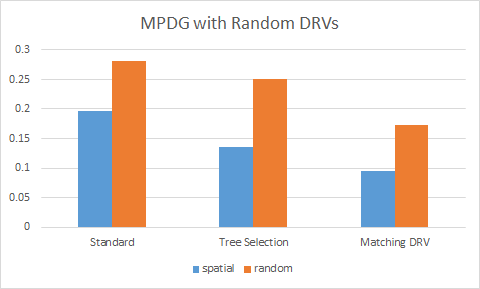
\includegraphics[width=.85\textwidth]{Figures/fullsysrand}
\end{center}
\caption{Full system test with random DRVs from uniform distribution}
\label{fig:fullsysrand}
\end{figure}

The real improvements came however from extreme queries which only use a small subset of dimensions.  The same parameters for our sytem were chosen with the exception of setting the DDD to 3, however the method of selecting the query DRVs was changed to only include a smaller subset of dimensions.  The method for doing so was to require a single dimension to be selected, and to determine whether or not other dimensions should be selected with a bernoulli random variable.  Thus, the distribution of the number of selected dimensions given a selection probability p and D dimensions is described by Binomial(D-1,p) + 1.  After selecting a subset of dimensions, the weight of each dimension was drawn randomly from a uniform distribution and normalized to a sum of one.  Of note is that when only one dimension is selected it will have a weight of 1 in the DRV, and it would be ideal to only split on that dimension.  Fortunitely, a seed DRV of all single dimension cases is included, and as such there is guaranteed to be a tree which perfectly matches, and only splits on that dimension.  In this case, the k-d tree performs equivalent to a binary search tree, and true nearest neighbors can be computed in O(Log(N)).  When more than one dimension is selected, while a perfect match tree likely won't exist (since weights are equal in seed DRVs), the two dimensional matching seed DRV will perform well if the query DRV is close to equal in the two dimensions, while the single dimension DRV will perform well when one dimension has a much larger weight than the other.

\begin{figure}[h]
\begin{center}
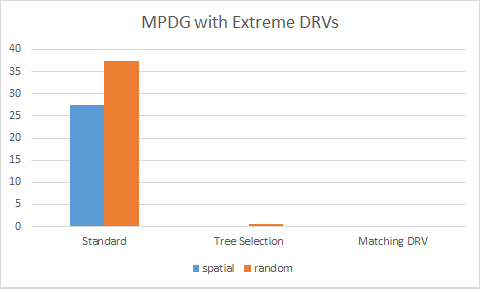
\includegraphics[width=.85\textwidth]{Figures/fullsysext}
\end{center}
\caption{Full system test with DRVs containing a low number of dimensions}
\label{fig:fullsysext}
\end{figure}

As shown in figure FILL, with extreme queries our data structure's performance was extremely close to the max possible performance with different DRVs, while the standard k-d tree performance decreased greatly.  Of course the true performance of our system likely lies somewhere in the middle of these cases shown in Figure FILL and FILL, as the true distribution of search queries likely lies somewhere in the middle.  Also of note is that seed DRVs with all sets of three dimensions were present, and nearly 85\% of the selected DRVs had three or less dimensions.  However, even when four to five dimensions are selected performance is still expected to be strong.

Because of the significantly higher performance of WSMS compared to SPM, future tests are performed only using the WSMS heuristic.  The key advantage to SPM is that all split dimensions are selected in constant time, wheras those in WSMS require a linear seek across all dimensions.  However, this cost is only associated with offline construction of the trees which is only performed once.  Since our benchmark attempts to optimize result quality on a live system, WSMS is a superior heuristic.  In \ref{sec:realworld}, we discuss that in a live system it may be necessary to reconstruct trees at times and as such, when performance tuning one should consider the merits of a heuristic with lower tree construction cost.

For future tests, unless otherwise specified, query DRVs were generated randomly with each dimension following the smae process used for the queries in Figure FILL.  Additionally, for future tests three different indexes were generated.  The first is a standard k-d tree for baseline performance.  The second is our system, using the standard parameters described above.  The final index generated is a singled k-d tree using WSMS with a seed DRV matching that of the query DRV.  This case represents hypothetical best case performance with our heuristics.

\section{Change of Dimensionality}

One important factor to test is how our system performs on data sets with different dimensionalities.  The dataset was again generated following the procedure from \ref{sec:inittest}; however, data was generated with different dimensions.

\begin{figure}[h]
\begin{center}
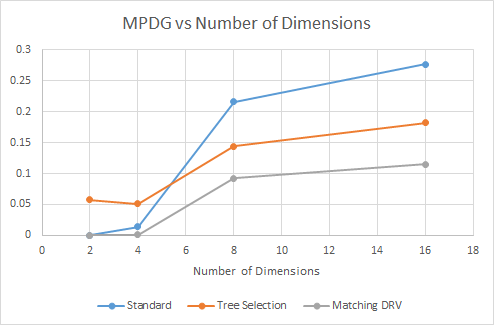
\includegraphics[width=.85\textwidth]{Figures/dims}
\end{center}
\caption{Full system test with data set of varying dimensions}
\label{fig:dim}
\end{figure}

The results for this test are shown in Figure FILL.  For each index, the MPDG increases with dimensionality.  This is to be expected, as performance for tree based indexes begins to degrade at higher dimensionalities.  Of note is that our system actually performed worse than a standard k-d tree for very low dimensionality.  This is likely because some searches were used to select the best trees.  Additionally, the k-d tree has the advantage of searching in a single tree, while searches in our index were split between multiple, and as seen in Figure FILL the performance of forests tends to be slightly worse than that of a single tree.  With a higher number of dimensions however, our system performs better than k-d trees, as the value of selecting trees with better seed DRVs is higher with more dimensions.

\section{Size of Dataset}

We also tested the performance of our system on datasets of varying size.  Again the same procedure from \ref{sec:inittest} was followed, but using a variety of different sizes.

\begin{figure}[h]
\begin{center}
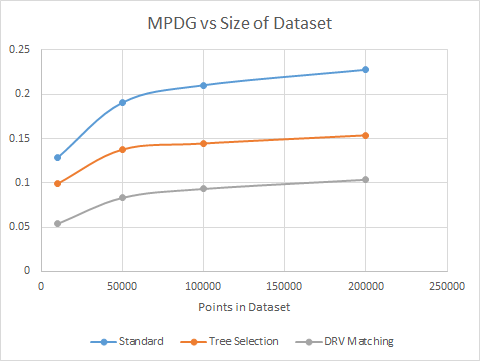
\includegraphics[width=.85\textwidth]{Figures/size}
\end{center}
\caption{Full system test with data set of varying size}
\label{fig:size}
\end{figure}

The results for this test are shown in Figure FILL.  For each of the indexes, the MPDG increases with the size of the dataset.  This is expected, as a larger dataset with a fixed number of nodes search means that a lower percentage of nodes are searched.  Of note is that the standard k-d tree index's performance decreased at a faster rate than that of our index and the tree with a matched seed DRV.  Thus, the benefits of our system are larger for bigger datasets. 

\section{Number of Trees}

The number of trees in our system is expected to have a direct impact on in its performance.  We tested our system against the same dataset described in \ref{sec:inittest}, generating our index with a varying number of random trees.

\begin{figure}[h]
\begin{center}
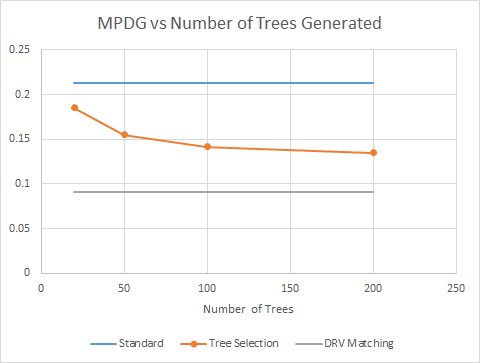
\includegraphics[width=.85\textwidth]{Figures/ntreesgen}
\end{center}
\caption{Full system test with varying number of random trees in our system}
\label{fig:ntreesgen}
\end{figure}

The results are shown in Figure FILL.  The orange line represents the performance of the standard k-d tree, while the grey line represents the performance of a tree with a matched seed DRV.  With a larger number of trees, the overall quality of of the selected trees will increase, since with more trees there are more chances for a high quality match.  However, this effect is diminishing.  As the number of trees increases, the performance increase from doing so drops.

\section{Nodes Searched}

\begin{figure}[h]
\begin{center}
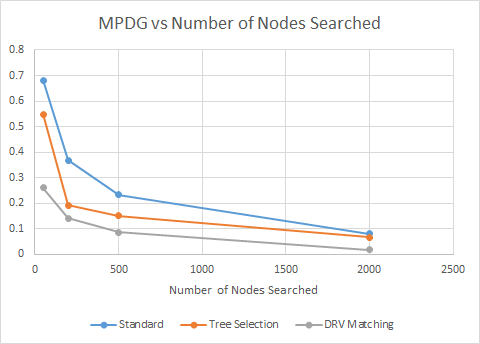
\includegraphics[width=.85\textwidth]{Figures/nsearch}
\end{center}
\caption{Full system test with varying number of nodes searched}
\label{fig:nsearch}
\end{figure}

We also considered the performance of our system for varying numbers of nodes searched.  The results for this test are shown in Figure FILL.  As expected, for each index, the MPDG decreases with an increase in the number of nodes searched.  This effect is dimishing however.  Initially, an increase in the number of nodes searched leads to a large decrease in MPDG, wheras a similar increase when a large number of nodes are already searched has little effect.  Also of importance is that for a very small number of nodes searched our system's performance is close to that of a standard k-d tree.  This is because a high proportion of the alloted searches are used to select which trees to search.  As the number of searches increases so does our system's performance relative to the standard k-d tree.  At a large enough number of searches, the standard k-d tree eventually catches up to our index.  Thus, our index was most effective when about .2\% to .5\% of the nodes were searched.

\section{Size of Result Set}

\begin{figure}[h]
\begin{center}
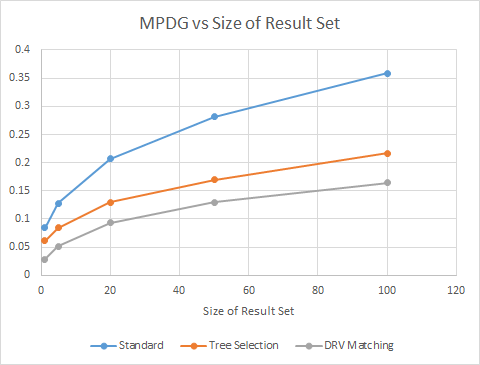
\includegraphics[width=.85\textwidth]{Figures/k}
\end{center}
\caption{Full system test with varying size of result set (K)}
\label{fig:kparam}
\end{figure}

\section{Number of Trees Per Query}

\begin{figure}[h]
\begin{center}
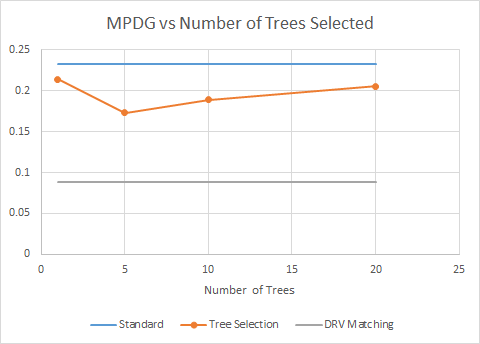
\includegraphics[width=.85\textwidth]{Figures/treesel}
\end{center}
\caption{Full system test with varying number of trees retrieved per query}
\label{fig:treesel}
\end{figure}

\section{Alternative Dataset}

http://archive.ics.uci.edu/ml/datasets/Corel+Image+Features
http://archive.ics.uci.edu/ml/machine-learning-databases/CorelFeatures-mld/CorelFeatures.data.html
\begin{figure}[h]
\begin{center}
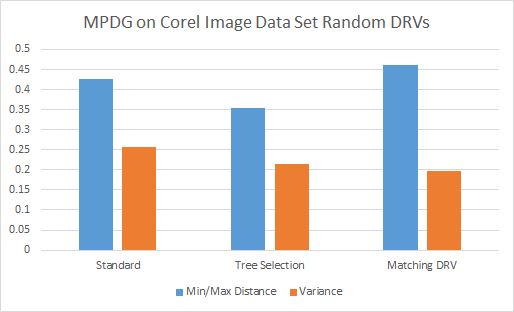
\includegraphics[width=.85\textwidth]{Figures/altrand}
\end{center}
\caption{Full system test on Corel Image Features Data Set with random DRVs from uniform distribution}
\label{fig:altrand}
\end{figure}

\begin{figure}[h]
\begin{center}
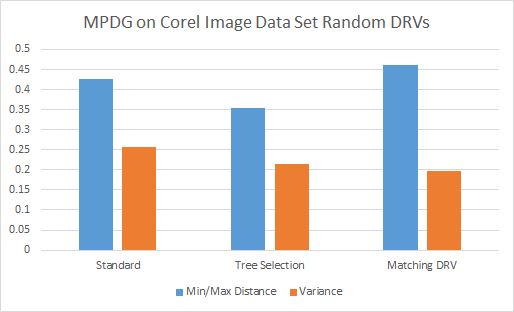
\includegraphics[width=.85\textwidth]{Figures/altext}
\end{center}
\caption{Full system test on Corel Image Features Data Set with DRVs with a low number of dimensions}
\label{fig:altext}
\end{figure}
check

\chapter{Conclusion} % Main chapter title

\label{conclusion} % For referencing the chapter elsewhere, use \ref{Chapter1} 

\lhead{Chapter 7. \emph{Conclusion}} % This is for the header on each page - perhaps a 

%% Chapter 1

\chapter{Chapter Title Here} % Main chapter title

\label{Chapter1} % For referencing the chapter elsewhere, use \ref{Chapter1} 

\lhead{Chapter 1. \emph{Chapter Title Here}} % This is for the header on each page - perhaps a shortened title

%----------------------------------------------------------------------------------------

\section{Welcome and Thank You}
Welcome to this \LaTeX{} Thesis Template, a beautiful and easy to use template for writing a thesis using the \LaTeX{} typesetting system.

If you are writing a thesis (or will be in the future) and its subject is technical or mathematical (though it doesn't have to be), then creating it in \LaTeX{} is highly recommended as a way to make sure you can just get down to the essential writing without having to worry over formatting or wasting time arguing with your word processor.

\LaTeX{} is easily able to professionally typeset documents that run to hundreds or thousands of pages long. With simple mark-up commands, it automatically sets out the table of contents, margins, page headers and footers and keeps the formatting consistent and beautiful. One of its main strengths is the way it can easily typeset mathematics, even \emph{heavy} mathematics. Even if those equations are the most horribly twisted and most difficult mathematical problems that can only be solved on a super-computer, you can at least count on \LaTeX{} to make them look stunning.

%----------------------------------------------------------------------------------------

\section{Learning \LaTeX{}}

\LaTeX{} is not a WYSIWYG (What You See is What You Get) program, unlike word processors such as Microsoft Word or Apple's Pages. Instead, a document written for \LaTeX{} is actually a simple, plain text file that contains \emph{no formatting}. You tell \LaTeX{} how you want the formatting in the finished document by writing in simple commands amongst the text, for example, if I want to use \textit{italic text for emphasis}, I write the `$\backslash$\texttt{textit}\{\}' command and put the text I want in italics in between the curly braces. This means that \LaTeX{} is a ``mark-up'' language, very much like HTML.

\subsection{A (not so short) Introduction to \LaTeX{}}

If you are new to \LaTeX{}, there is a very good eBook -- freely available online as a PDF file -- called, ``The Not So Short Introduction to \LaTeX{}''. The book's title is typically shortened to just ``lshort''. You can download the latest version (as it is occasionally updated) from here:\\
\href{http://www.ctan.org/tex-archive/info/lshort/english/lshort.pdf}{\texttt{http://www.ctan.org/tex-archive/info/lshort/english/lshort.pdf}}

It is also available in several other languages. Find yours from the list on this page:\\
\href{http://www.ctan.org/tex-archive/info/lshort/}{\texttt{http://www.ctan.org/tex-archive/info/lshort/}}

It is recommended to take a little time out to learn how to use \LaTeX{} by creating several, small `test' documents. Making the effort now means you're not stuck learning the system when what you \emph{really} need to be doing is writing your thesis.

\subsection{A Short Math Guide for \LaTeX{}}

If you are writing a technical or mathematical thesis, then you may want to read the document by the AMS (American Mathematical Society) called, ``A Short Math Guide for \LaTeX{}''. It can be found online here:\\
\href{http://www.ams.org/tex/amslatex.html}{\texttt{http://www.ams.org/tex/amslatex.html}}\\
under the ``Additional Documentation'' section towards the bottom of the page.

\subsection{Common \LaTeX{} Math Symbols}
There are a multitude of mathematical symbols available for \LaTeX{} and it would take a great effort to learn the commands for them all. The most common ones you are likely to use are shown on this page:\\
\href{http://www.sunilpatel.co.uk/latexsymbols.html}{\texttt{http://www.sunilpatel.co.uk/latexsymbols.html}}

You can use this page as a reference or crib sheet, the symbols are rendered as large, high quality images so you can quickly find the \LaTeX{} command for the symbol you need.

\subsection{\LaTeX{} on a Mac}
 
The \LaTeX{} package is available for many systems including Windows, Linux and Mac OS X. The package for OS X is called MacTeX and it contains all the applications you need -- bundled together and pre-customised -- for a fully working \LaTeX{} environment and workflow.
 
MacTeX includes a dedicated \LaTeX{} IDE (Integrated Development Environment) called ``TeXShop'' for writing your `\texttt{.tex}' files and ``BibDesk'': a program to manage your references and create your bibliography section just as easily as managing songs and creating playlists in iTunes.

%----------------------------------------------------------------------------------------

\section{Getting Started with this Template}

If you are familiar with \LaTeX{}, then you can familiarise yourself with the contents of the Zip file and the directory structure and then place your own information into the `\texttt{Thesis.cls}' file. Section \ref{FillingFile} on page \pageref{FillingFile} tells you how to do this. Make sure you read section \ref{ThesisConventions} about thesis conventions to get the most out of this template and then get started with the `\texttt{Thesis.tex}' file straightaway.

If you are new to \LaTeX{} it is recommended that you carry on reading through the rest of the information in this document.

\subsection{About this Template}

This \LaTeX{} Thesis Template is originally based and created around a \LaTeX{} style file created by Steve R.\ Gunn from the University of Southampton (UK), department of Electronics and Computer Science. You can find his original thesis style file at his site, here:\\
\href{http://www.ecs.soton.ac.uk/~srg/softwaretools/document/templates/}{\texttt{http://www.ecs.soton.ac.uk/$\sim$srg/softwaretools/document/templates/}}

My thesis originally used the `\texttt{ecsthesis.cls}' from his list of styles. However, I knew \LaTeX{} could still format better. To get the look I wanted, I modified his style and also created a skeleton framework and folder structure to place the thesis files in.

This Thesis Template consists of that modified style, the framework and the folder structure. All the work that has gone into the preparation and groundwork means that all you have to bother about is the writing.

Before you begin using this template you should ensure that its style complies with the thesis style guidelines imposed by your institution. In most cases this template style and layout will be suitable. If it is not, it may only require a small change to bring the template in line with your institution's recommendations.

%----------------------------------------------------------------------------------------

\section{What this Template Includes}

\subsection{Folders}

This template comes as a single Zip file that expands out to many files and folders. The folder names are mostly self-explanatory:

\textbf{Appendices} -- this is the folder where you put the appendices. Each appendix should go into its own separate `\texttt{.tex}' file. A template is included in the directory.

\textbf{Chapters} -- this is the folder where you put the thesis chapters. A thesis usually has about seven chapters, though there is no hard rule on this. Each chapter should go in its own separate `\texttt{.tex}' file and they usually are split as:
\begin{itemize}
\item Chapter 1: Introduction to the thesis topic
\item Chapter 2: Background information and theory
\item Chapter 3: (Laboratory) experimental setup
\item Chapter 4: Details of experiment 1
\item Chapter 5: Details of experiment 2
\item Chapter 6: Discussion of the experimental results
\item Chapter 7: Conclusion and future directions
\end{itemize}
This chapter layout is specialised for the experimental sciences.

\textbf{Figures} -- this folder contains all figures for the thesis. These are the final images that will go into the thesis document.

\textbf{Primitives} -- this is the folder that contains scraps, particularly because one final image in the `Figures' folder may be made from many separate images and photos, these source images go here. This keeps the intermediate files separate from the final thesis figures.

\subsection{Files}

Included are also several files, most of them are plain text and you can see their contents in a text editor. Luckily, many of them are auxiliary files created by \LaTeX{} or BibTeX and which you don't need to bother about:

\textbf{Bibliography.bib} -- this is an important file that contains all the bibliographic information and references that you will be citing in the thesis for use with BibTeX. You can write it manually, but there are reference manager programs available that will create and manage it for you. Bibliographies in \LaTeX{} are a large subject and you may need to read about BibTeX before starting with this.

\textbf{Thesis.cls} -- this is an important file. It is the style file that tells \LaTeX{} how to format the thesis. You will also need to open this file in a text editor and fill in your own information (such as name, department, institution). Luckily, this is not too difficult and is explained in section \ref{FillingFile} on page \pageref{FillingFile}.

\textbf{Thesis.pdf} -- this is your beautifully typeset thesis (in the PDF file format) created by \LaTeX{}.

\textbf{Thesis.tex} -- this is an important file. This is the file that you tell \LaTeX{} to compile to produce your thesis as a PDF file. It contains the framework and constructs that tell \LaTeX{} how to layout the thesis. It is heavily commented so you can read exactly what each line of code does and why it is there. After you put your own information into the `\texttt{Thesis.cls}' file, go to this file and begin filling it in -- you have now started your thesis!

\textbf{vector.sty} -- this is a \LaTeX{} package, it tells \LaTeX{} how to typeset mathematical vectors. Using this package is very easy and you can read the documentation on the site (you just need to look at the `\texttt{vector.pdf}' file):\\
\href{http://www.ctan.org/tex-archive/macros/latex/contrib/vector/}{\texttt{http://www.ctan.org/tex-archive/macros/latex/contrib/vector/}}

\textbf{lstpatch.sty} -- this is a \LaTeX{} package required by this LaTeX template and is included as not all \TeX{} distributions have it installed by default. You do not need to modify this file.

Files that are \emph{not} included, but are created by \LaTeX{} as auxiliary files include:

\textbf{Thesis.aux} -- this is an auxiliary file generated by \LaTeX{}, if it is deleted \LaTeX{} simply regenerates it when you run the main `\texttt{.tex}' file.

\textbf{Thesis.bbl} -- this is an auxiliary file generated by BibTeX, if it is deleted, BibTeX simply regenerates it when you run the main tex file. Whereas the `\texttt{.bib}' file contains all the references you have, this `\texttt{.bbl}' file contains the references you have actually cited in the thesis and is used to build the bibliography section of the thesis.

\textbf{Thesis.blg} -- this is an auxiliary file generated by BibTeX, if it is deleted BibTeX simply regenerates it when you run the main `\texttt{.tex}' file.

\textbf{Thesis.lof} -- this is an auxiliary file generated by \LaTeX{}, if it is deleted \LaTeX{} simply regenerates it when you run the main `\texttt{.tex}' file. It tells \LaTeX{} how to build the `List of Figures' section.

\textbf{Thesis.log} -- this is an auxiliary file generated by \LaTeX{}, if it is deleted \LaTeX{} simply regenerates it when you run the main `\texttt{.tex}' file. It contains messages from \LaTeX{}, if you receive errors and warnings from \LaTeX{}, they will be in this `\texttt{.log}' file.

\textbf{Thesis.lot} -- this is an auxiliary file generated by \LaTeX{}, if it is deleted \LaTeX{} simply regenerates it when you run the main `\texttt{.tex}' file. It tells \LaTeX{} how to build the `List of Tables' section.

\textbf{Thesis.out} -- this is an auxiliary file generated by \LaTeX{}, if it is deleted \LaTeX{} simply regenerates it when you run the main `\texttt{.tex}' file.


So from this long list, only the files with the `\texttt{.sty}', `\texttt{.bib}', `\texttt{.cls}' and `\texttt{.tex}' extensions are the most important ones. The other auxiliary files can be ignored or deleted as \LaTeX{} and BibTeX will regenerate them.

%----------------------------------------------------------------------------------------

\section{Filling in the `\texttt{Thesis.cls}' File}\label{FillingFile}

You will need to personalise the thesis template and make it your own by filling in your own information. This is done by editing the `\texttt{Thesis.cls}' file in a text editor.

Open the file and scroll down, past all the `$\backslash$\texttt{newcommand}\ldots' items until you see the entries for `\texttt{University Name}', `\texttt{Department Name}', etc\ldots.

Fill out the information about your group and institution and ensure you keep to block capitals where it asks you to. You can also insert web links, if you do, make sure you use the full URL, including the `\texttt{http://}' for this.

The last item you should need to fill in is the Faculty Name (in block capitals). When you have done this, save the file and recompile `\texttt{Thesis.tex}'. All the information you filled in should now be in the PDF, complete with web links. You can now begin your thesis proper!

%----------------------------------------------------------------------------------------

\section{The `\texttt{Thesis.tex}' File Explained}

The \texttt{Thesis.tex} file contains the structure of the thesis. There are plenty of written comments that explain what pages, sections and formatting the \LaTeX{} code is creating. Initially there seems to be a lot of \LaTeX{} code, but this is all formatting, and it has all been taken care of so you don't have to do it.

Begin by checking that your information on the title page is correct. For the thesis declaration, your institution may insist on something different than the text given. If this is the case, just replace what you see with what is required.

Then comes a page which contains a funny quote. You can put your own, or quote your favourite scientist, author, person, etc\ldots Make sure to put the name of the person who you took the quote from.

Next comes the acknowledgements. On this page, write about all the people who you wish to thank (not forgetting parents, partners and your advisor/supervisor).

The contents pages, list of figures and tables are all taken care of for you and do not need to be manually created or edited. The next set of pages are optional and can be deleted since they are for a more technical thesis: insert a list of abbreviations you have used in the thesis, then a list of the physical constants and numbers you refer to and finally, a list of mathematical symbols used in any formulae. Making the effort to fill these tables means the reader has a one-stop place to refer to instead of searching the internet and references to try and find out what you meant by certain abbreviations or symbols.

The list of symbols is split into the Roman and Greek alphabets. Whereas the abbreviations and symbols ought to be listed in alphabetical order (and this is \emph{not} done automatically for you) the list of physical constants should be grouped into similar themes.

The next page contains a one line dedication. Who will you dedicate your thesis to?

Finally, there is the section where the chapters are included. Uncomment the lines (delete the `\texttt{\%}' character) as you write the chapters. Each chapter should be written in its own file and put into the `Chapters' folder and named `\texttt{Chapter1}', `\texttt{Chapter2}, etc\ldots Similarly for the appendices, uncomment the lines as you need them. Each appendix should go into its own file and placed in the `Appendices' folder.

After the preamble, chapters and appendices finally comes the bibliography. The bibliography style (called `\texttt{unsrtnat}') is used for the bibliography and is a fully featured style that will even include links to where the referenced paper can be found online. Do not under estimate how grateful you reader will be to find that a reference to a paper is just a click away. Of course, this relies on you putting the URL information into the BibTeX file in the first place.

%----------------------------------------------------------------------------------------

\section{Thesis Features and Conventions}\label{ThesisConventions}

To get the best out of this template, there are a few conventions that you may want to follow.

One of the most important (and most difficult) things to keep track of in such a long document as a thesis is consistency. Using certain conventions and ways of doing things (such as using a Todo list) makes the job easier. Of course, all of these are optional and you can adopt your own method.

\subsection{Printing Format}

This thesis template is designed for single sided printing as most theses are printed and bound this way. This means that the left margin is always wider than the right (for binding). Four out of five people will now judge the margins by eye and think, ``I never 
noticed that before.''.

The headers for the pages contain the page number on the right side (so it is easy to flick through to the page you want) and the chapter name on the left side.

The text is set to 11 point and a line spacing of 1.3. Generally, it is much more readable to have a smaller text size and wider gap between the lines than it is to have a larger text size and smaller gap. Again, you can tune the text size and spacing should you want or need to. The text size can be set in the options for the `$\backslash$\texttt{documentclass}' command at the top of the `\texttt{Thesis.tex}' file and the spacing can be changed by setting a different value in the `$\backslash$\texttt{setstretch}' commands (scattered throughout the `\texttt{Thesis.tex}' file).

\subsection{Using US Letter Paper}

The paper size used in the template is A4, which is a common -- if not standard -- size in Europe. If you are using this thesis template elsewhere and particularly in the United States, then you may have to change the A4 paper size to the US Letter size. Unfortunately, this is not as simple as replacing instances of `\texttt{a4paper}' with `\texttt{letterpaper}'.

This is because the final PDF file is created directly from the \LaTeX{} source using a program called `\texttt{pdfTeX}' and in certain conditions, paper size commands are ignored and all documents are created with the paper size set to the size stated in the configuration file for pdfTeX (called `\texttt{pdftex.cfg}').

What needs to be done is to change the paper size in the configuration file for \texttt{pdfTeX} to reflect the letter size. There is an excellent tutorial on how to do this here: \\
\href{http://www.physics.wm.edu/~norman/latexhints/pdf_papersize.html}{\texttt{http://www.physics.wm.edu/$\sim$norman/latexhints/pdf\_papersize.html}}

It may be sufficient just to replace the dimensions of the A4 paper size with the US Letter size in the \texttt{pdftex.cfg} file. Due to the differences in the paper size, the resulting margins may be different to what you like or require (as it is common for Institutions to dictate certain margin sizes). If this is the case, then the margin sizes can be tweaked by opening up the \texttt{Thesis.cls} file and searching for the line beginning with, `$\backslash$\texttt{setmarginsrb}' (not very far down from the top), there you will see the margins specified. Simply change those values to what you need (or what looks good) and save. Now your document should be set up for US Letter paper size with suitable margins.

\subsection{References}

The `\texttt{natbib}' package is used to format the bibliography and inserts references such as this one \citep{Reference3}. The options used in the `\texttt{Thesis.tex}' file mean that the references are listed in numerical order as they appear in the text. Multiple references are rearranged in numerical order (e.g. \citep{Reference2, Reference1}) and multiple, sequential references become reformatted to a reference range (e.g. \citep{Reference2, Reference1, Reference3}). This is done automatically for you. To see how you use references, have a look at the `\texttt{Chapter1.tex}' source file. Many reference managers allow you to simply drag the reference into the document as you type.

Scientific references should come \emph{before} the punctuation mark if there is one (such as a comma or period). The same goes for footnotes\footnote{Such as this footnote, here down at the bottom of the page.}. You can change this but the most important thing is to keep the convention consistent throughout the thesis. Footnotes themselves should be full, descriptive sentences (beginning with a capital letter and ending with a full stop).

To see how \LaTeX{} typesets the bibliography, have a look at the very end of this document (or just click on the reference number links).

\subsection{Figures}

There will hopefully be many figures in your thesis (that should be placed in the `Figures' folder). The way to insert figures into your thesis is to use a code template like this:
\begin{verbatim}
\begin{figure}[htbp]
  \centering
    
\includegraphics{./Figures/Electron.pdf}
    \rule{35em}{0.5pt}
  \caption[An Electron]{An electron (artist's impression).}
  \label{fig:Electron}
\end{figure}
\end{verbatim}
Also look in the source file. Putting this code into the source file produces the picture of the electron that you can see in the figure below.

\begin{figure}[htbp]
	\centering
		
\includegraphics{./Figures/Electron.pdf}
		\rule{35em}{0.5pt}
	\caption[An Electron]{An electron (artist's impression).}
	\label{fig:Electron}
\end{figure}

Sometimes figures don't always appear where you write them in the source. The placement depends on how much space there is on the page for the figure. Sometimes there is not enough room to fit a figure directly where it should go (in relation to the text) and so \LaTeX{} puts it at the top of the next page. Positioning figures is the job of \LaTeX{} and so you should only worry about making them look good!

Figures usually should have labels just in case you need to refer to them (such as in Figure \ref{fig:Electron}). The `$\backslash$\texttt{caption}' command contains two parts, the first part, inside the square brackets is the title that will appear in the `List of Figures', and so should be short. The second part in the curly brackets should contain the longer and more descriptive caption text.

The `$\backslash$\texttt{rule}' command is optional and simply puts an aesthetic horizontal line below the image. If you do this for one image, do it for all of them.

The \LaTeX{} Thesis Template is able to use figures that are either in the PDF or JPEG file format.

\subsection{Typesetting mathematics}

If your thesis is going to contain heavy mathematical content, be sure that \LaTeX{} will make it look beautiful, even though it won't be able to solve the equations for you.

The ``Not So Short Introduction to \LaTeX{}'' (available \href{http://www.ctan.org/tex-archive/info/lshort/english/lshort.pdf}{here}) should tell you everything you need to know for most cases of typesetting mathematics. If you need more information, a much more thorough mathematical guide is available from the AMS called, ``A Short Math Guide to \LaTeX{}'' and can be downloaded from:\\
\href{ftp://ftp.ams.org/pub/tex/doc/amsmath/short-math-guide.pdf}{\texttt{ftp://ftp.ams.org/pub/tex/doc/amsmath/short-math-guide.pdf}}

There are many different \LaTeX{} symbols to remember, luckily you can find the most common symbols \href{http://www.sunilpatel.co.uk/latexsymbols.html}{here}. You can use the web page as a quick reference or crib sheet and because the symbols are grouped and rendered as high quality images (each with a downloadable PDF), finding the symbol you need is quick and easy.

You can write an equation, which is automatically given an equation number by \LaTeX{} like this:
\begin{verbatim}
\begin{equation}
E = mc^{2}
  \label{eqn:Einstein}
\end{equation}
\end{verbatim}

This will produce Einstein's famous energy-matter equivalence equation:
\begin{equation}
E = mc^{2}
\label{eqn:Einstein}
\end{equation}

All equations you write (which are not in the middle of paragraph text) are automatically given equation numbers by \LaTeX{}. If you don't want a particular equation numbered, just put the command, `$\backslash$\texttt{nonumber}' immediately after the equation.

%----------------------------------------------------------------------------------------

\section{Sectioning and Subsectioning}

You should break your thesis up into nice, bite-sized sections and subsections. \LaTeX{} automatically builds a table of Contents by looking at all the `$\backslash$\texttt{chapter}$\{\}$', `$\backslash$\texttt{section}$\{\}$' and `$\backslash$\texttt{subsection}$\{\}$' commands you write in the source.

The table of Contents should only list the sections to three (3) levels. A `$\backslash$\texttt{chapter}$\{\}$' is level one (1). A `$\backslash$\texttt{section}$\{\}$' is level two (2) and so a `$\backslash$\texttt{subsection}$\{\}$' is level three (3). In your thesis it is likely that you will even use a `$\backslash$\texttt{subsubsection}$\{\}$', which is level four (4). Adding all these will create an unnecessarily cluttered table of Contents and so you should use the `$\backslash$\texttt{subsubsection$^{*}\{\}$}' command instead (note the asterisk). The asterisk ($^{*}$) tells \LaTeX{} to omit listing the subsubsection in the Contents, keeping it clean and tidy.

%----------------------------------------------------------------------------------------

\section{In Closing}

You have reached the end of this mini-guide. You can now rename or overwrite this pdf file and begin writing your own `\texttt{Chapter1.tex}' and the rest of your thesis. The easy work of setting up the structure and framework has been taken care of for you. It's now your job to fill it out!

Good luck and have lots of fun!

\begin{flushright}
Guide written by ---\\
Sunil Patel: \href{http://www.sunilpatel.co.uk}{www.sunilpatel.co.uk}
\end{flushright}
%\input{./Chapters/Chapter2} 
%\input{./Chapters/Chapter3}
%\input{./Chapters/Chapter4} 
%\input{./Chapters/Chapter5} 
%\input{./Chapters/Chapter6} 
%\input{./Chapters/Chapter7} 

%----------------------------------------------------------------------------------------
%	THESIS CONTENT - APPENDICES
%----------------------------------------------------------------------------------------

\addtocontents{toc}{\vspace{2em}} % Add a gap in the Contents, for aesthetics

\appendix % Cue to tell LaTeX that the following 'chapters' are Appendices

% Include the appendices of the thesis as separate files from the Appendices folder
% Uncomment the lines as you write the Appendices

% Appendix A

\chapter{Appendix Title Here} % Main appendix title

\label{AppendixA} % For referencing this appendix elsewhere, use \ref{AppendixA}

\lhead{Appendix A. \emph{Appendix Title Here}} % This is for the header on each page - perhaps a shortened title

Write your Appendix content here.
%\input{./Appendices/AppendixB}
%\input{./Appendices/AppendixC}

\addtocontents{toc}{\vspace{2em}} % Add a gap in the Contents, for aesthetics

\backmatter

%----------------------------------------------------------------------------------------
%	BIBLIOGRAPHY
%----------------------------------------------------------------------------------------

\label{Bibliography}

\lhead{\emph{Bibliography}} % Change the page header to say "Bibliography"

\bibliographystyle{unsrtnat} % Use the "unsrtnat" BibTeX style for formatting the Bibliography

\bibliography{Bibliography} % The references (bibliography) information are stored in the file named "Bibliography.bib"

\end{document}